\documentclass[10pt, a5paper]{article}
\usepackage{pdfpages}
\usepackage{parallel}
\usepackage[T2A]{fontenc}
\usepackage{ucs}
\usepackage[utf8x]{inputenc}
\usepackage[polish,english,russian]{babel}
\usepackage{hyperref}
\usepackage{rotating}
\usepackage[inner=2cm,top=1.8cm,outer=2cm,bottom=2.3cm,nohead]{geometry}
\usepackage{listings}
\usepackage{graphicx}
\usepackage{wrapfig}
\usepackage{longtable}
\usepackage{indentfirst}
\usepackage{array}
\newcolumntype{P}[1]{>{\raggedright\arraybackslash}p{#1}}
\frenchspacing
\usepackage{fixltx2e} %text sub- and superscripts
\usepackage{icomma} % коскі ў матэматычным рэжыме
\PreloadUnicodePage{4}

\newcommand{\longpage}{\enlargethispage{\baselineskip}}
\newcommand{\shortpage}{\enlargethispage{-\baselineskip}}

\def\switchlang#1{\expandafter\csname switchlang#1\endcsname}
\def\switchlangbe{
\let\saverefname=\refname%
\def\refname{Літаратура}%
\def\figurename{Іл.}%
}
\def\switchlangen{
\let\saverefname=\refname%
\def\refname{References}%
\def\figurename{Fig.}%
}
\def\switchlangru{
\let\saverefname=\refname%
\let\savefigurename=\figurename%
\def\refname{Литература}%
\def\figurename{Рис.}%
}

\hyphenation{admi-ni-stra-tive}
\hyphenation{ex-pe-ri-ence}
\hyphenation{fle-xi-bi-li-ty}
\hyphenation{Py-thon}
\hyphenation{ma-the-ma-ti-cal}
\hyphenation{re-ported}
\hyphenation{imp-le-menta-tions}
\hyphenation{pro-vides}
\hyphenation{en-gi-neering}
\hyphenation{com-pa-ti-bi-li-ty}
\hyphenation{im-pos-sible}
\hyphenation{desk-top}
\hyphenation{elec-tro-nic}
\hyphenation{com-pa-ny}
\hyphenation{de-ve-lop-ment}
\hyphenation{de-ve-loping}
\hyphenation{de-ve-lop}
\hyphenation{da-ta-ba-se}
\hyphenation{plat-forms}
\hyphenation{or-ga-ni-za-tion}
\hyphenation{pro-gramming}
\hyphenation{in-stru-ments}
\hyphenation{Li-nux}
\hyphenation{sour-ce}
\hyphenation{en-vi-ron-ment}
\hyphenation{Te-le-pathy}
\hyphenation{Li-nux-ov-ka}
\hyphenation{Open-BSD}
\hyphenation{Free-BSD}
\hyphenation{men-ti-on-ed}
\hyphenation{app-li-ca-tion}

\def\progref!#1!{\texttt{#1}}
\renewcommand{\arraystretch}{2} %Іначай формулы ў матрыцы зліпаюцца з лініямі
\usepackage{array}

\def\interview #1 (#2), #3, #4, #5\par{

\section[#1, #3, #4]{#1 -- #3, #4}
\def\qname{LVEE}
\def\aname{#1}
\def\q ##1\par{{\noindent \bf \qname: ##1 }\par}
\def\a{{\noindent \bf \aname: } \def\qname{L}\def\aname{#2}}
}

\def\interview* #1 (#2), #3, #4, #5\par{

\section*{#1\\{\small\rm #3, #4. #5}}

\def\qname{LVEE}
\def\aname{#1}
\def\q ##1\par{{\noindent \bf \qname: ##1 }\par}
\def\a{{\noindent \bf \aname: } \def\qname{L}\def\aname{#2}}
}

\switchlang{en}
\begin{document}
\title{First steps into OpenStack\footnote{\url{perepiolkin@itspartner.net}, \url{http://lvee.org/ru/abstracts/217}}}
\author{Andrei Perapiolkin, Minsk, Belarus}
\maketitle
\begin{abstract}
This report aims to give understanding of what OpenStack is, moreover to guide on how to start to use and contribute to the OpenStack. I will describe OpenStack in the context of distributed computing; give short description of OpenStack services Nova, Neutron, Cinder, Swift, Glance, Horisont, Keystone; give short description of devstack, packstack, suseCloud, ubuntu juju. On the example of the devstack, I will give a short description of how you can deploy your own OpenStack cloud.
\end{abstract}


New technologies in the IT world mostly appear on the basis of existing knowledge approaches and infrastructure. It is also true for the cloud computing. We can see that new step of evolution of the grid and cluster systems is Cloud Computing systems. The reason of evolution is high demand for the available computing resources in the society. Rapidly changing modern world requires fast speed deployment of the IT infrastructure. This determines fast deployment of business infrastructure -- fast accessibility to the computing resources, storage, ready software deployments, and others. From the perspective of the people who offer all of these resources it is extremely important to have orchestration tools to control and automate all of these tasks. So the merger of all of the requirements leaded to the appearance of the OpenStack.

OpenStack is a merge of separate already existing technologies under the hood of Python automation. It provides such technology components like:

\begin{itemize}
  \item \textbf{Keystone} provides an authentication and authorization service for other OpenStack services. Provides a catalog of endpoints for all OpenStack services.
  \item \textbf{Nova} manages the computational resources by creating virtual computation environments.
  \item \textbf{Neutron} enables network connectivity for the OpenStack services. It allows to define networks, their topology, and attach instances.
  \item \textbf{Cinder} provides persistent block storage to running instances.
  \item \textbf{Glance} stores images for the Nova. Allowing it to make quick start from prepared image deployment.
  \item \textbf{Swift} stores and retrieves arbitrary unstructured data objects via REST API.
  \item \textbf{Horison} service provides web-based interface, and allows to \linebreak interact with OpenStack services like Cinder, Nova…
\end{itemize}

\begin{figure}[h!]
  \centering
  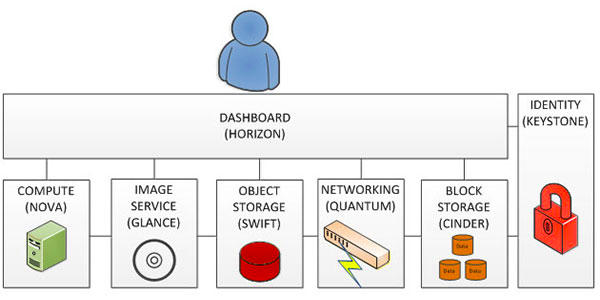
\includegraphics[width=10cm]{19_2016_Perapiolkin1.png}
\end{figure}

There are also such services like \textbf{Ceilometer} (provides telemetry), \textbf{Trove} (interaction with database), \textbf{Manila} (provides shared file \linebreak system) and some others…

For instance, \textbf{Nova} which serves as a computational resource \linebreak provider by itself is a management that aggregates emulation, \linebreak visualization and containerization solutions under the unified API. Nova works with KVM, QEMU, Vmware ESXi, Microsoft Hyper-V, \linebreak XenServer, Docker and others.

Сore OpenStack service deployment process is a complex  task. In bare OpenStack deployment it’s get done by consistent configuration of each servicein in the manner that allows them to interact in between. This task can be simplified by using existing deployment automation tools like devstack and packstack. After installation and configuration admin can validate solution by running Tempest tests.

\begin{thebibliography}{99}
\bibitem{Perapiolkin1} OpenStack \url{https://www.openstack.org/}
\bibitem{Perapiolkin2} Nova \url{https://wiki.openstack.org/wiki/Nova}
\bibitem{Perapiolkin3} devstack \url{http://docs.openstack.org/developer/devstack/}
\bibitem{Perapiolkin4} RDO \url{https://www.rdoproject.org/}
\bibitem{Perapiolkin5} OpenStack diagram \url{http://www.ca.com/us/lpg/ca-}\linebreak\url{technology-exchange/sunny-outlook-for-openstack-clouds.aspx}
\end{thebibliography}
\end{document}
